\documentclass[]{beamer}
\newcommand{\R}{\textbf{R}}
\newcommand{\dee}{\;\text{d}}
\newcommand{\eps}{\varepsilon}
\newcommand{\pl}[2]{\frac{\partial #1}{\partial #2}}
\newcommand{\dl}[2]{\frac{\text{d} #1}{\text{d} #2}}
\newcommand{\sgn}{\text{sgn}}
\newcommand{\bigoh}{\mathcal{O}}

\usepackage{etoolbox}
\usepackage{booktabs}
\newtoggle{handout}
\togglefalse{handout}

\iftoggle{handout}{
	\usepackage{pgfpages}
	\pgfpagesuselayout{4 on 1}[border shrink=5mm]
}{}

\usepackage{tikz}
\usetikzlibrary{arrows.meta}
\usepackage{xcolor}
\usepackage{mathtools}

\usetikzlibrary{positioning,arrows.meta}

\title{6.3 Exponential Functions}
\author{Math 6010}
\institute{9-27-2023}
\date{}

\setbeamertemplate{footline}
{
	\hbox{\begin{beamercolorbox}[wd=1\paperwidth,ht=2.25ex,dp=1ex,right]{framenumber}%
			\usebeamerfont{framenumber}\insertframenumber{} / \inserttotalframenumber\hspace*{2ex}
	\end{beamercolorbox}}%
	\vskip0pt%
}

\usefonttheme{serif}

\setbeamertemplate{blocks}[rounded][shadow=true]
\setbeamercolor{frametitle}{fg=black,bg=blue!20!white}
\setbeamercolor{block title}{bg=blue!20!white,fg=black}
\setbeamercolor{block body}{bg=blue!10}


\begin{document}
	\beamertemplatenavigationsymbolsempty
	
	\frame{\titlepage}
	
%	\begin{frame}{Review of Exponents}
%		Let $a > 0$ and $m, n$ be integers
%		\vspace*{1em}
%		
%		$a^m = \underbrace{a \cdot a \cdot\ldots \cdot a}_{m \text{ times}}$ \pause \qquad $(1.5)^3 = 1.5 \cdot 1.5 \cdot 1.5 = 3.375$
%		\vspace*{1em}
%		\pause
%		\begin{itemize}
%			\item $a^0 = 1$,\quad $1^m = 1$, \quad $a^1 = a$
%			\pause
%			\vfill
%			\item $a^m \cdot a^n = a^{m+n}$ \pause \qquad $\underbrace{a\cdot a\cdot\ldots\cdot a}_{m\text{ times}} \cdot \underbrace{a\cdot a\cdot\ldots\cdot a}_{n\text{ times}}$
%			\vfill
%			\pause
%			\item $\frac{1}{a^n} = a^{-n}$ \pause \qquad want $a^{-n}\cdot a^n = a^0 = 1$
%			\vfill
%			\pause
%			\item $\frac{a^m}{a^n} = a^{m-n}$
%			\vfill
%			\pause
%			\item $\left(a^n\right)^m = a^{m\cdot n}$ \qquad $\underbrace{a^n \cdot a^n \cdot \ldots \cdot a^n}_{m\text{ times}}$
%			\vfill
%			\pause
%			\item $a^\frac{1}{n} = \sqrt[n]{a}$ \qquad want $\left(a^\frac{1}{n}\right)^n = a^1 = a$
%			\vfill
%			\pause 
%			\item $a^\frac{m}{n} = \sqrt[n]{a^m}$
%		\end{itemize}
%	\end{frame}
	
	\begin{frame}{Objectives}
		\begin{itemize}
			\item Define exponential functions ($f(x) = C\cdot a^x$)
			\pause\vfill
			\item Graph exponential functions
			\pause\vfill
			\item Understand basic properties of exponential functions
		\end{itemize}
	\end{frame}
	
	\begin{frame}{Extended Exponents}
		Want a function like
		\begin{equation*}
			f(x) = C\cdot a^x
		\end{equation*}
		\pause
		Recall: if $x = \frac{m}{n}$, then $a^x = a^\frac{m}{n} = \sqrt[n]{a^m}$
		\pause
		\vfill
		But $x$ might not be $\frac{m}{n}$, for integers $m,n$...
		\pause\vfill
		\begin{itemize}
			\item $x = \pi, \sqrt{2}$, and so on
		\end{itemize}
		\pause
		\vfill
		...but \textit{every} number has a decimal expansion
		\begin{equation*}
			\frac{2}{5} = 0.4, \qquad \frac{1}{3} = 0.3333..., \qquad \pi=3.14159..., \qquad \sqrt{2} = 1.41421...
		\end{equation*}
		\pause\vfill
		Approximate any number $x$ by \textit{finitely many} of its decimal digits.
		\begin{equation*}
			a^\pi \approx a^{3.14} = a^{\frac{314}{100}} = \sqrt[100]{a^{314}}
		\end{equation*}
	\end{frame}

	\begin{frame}{Extended Exponents}
		The more digits we use, the closer we get to the true value of $a^\pi$
		\vfill
		\begin{center}
		\begin{tabular}{@{}lllllcl@{}}
			$2^3$ & $2^{3.1}$ & $2^{3.14}$ & $2^{3.141}$ & $2^{3.1415}$ & $\cdots$ & $2^\pi$\\
			\midrule
			8.0000 & 8.5742 & 8.8152 & 8.8213 & 8.8244 & $\cdots$ & 8.8250
		\end{tabular}
		\end{center}
		\pause
		\vfill
		So we can use any number $x$ in the exponent. Hooray!
		\pause
		\vfill
		Better still, we get to keep all the properties of exponents that we already know:
		\begin{block}{Exponent Properties}
			If $x,y$ are \textit{any real numbers}, and $a,b > 0$, then
			\begin{alignat*}{3}
				&\bullet a^x\cdot a^y = a^{x+y} &\quad &\bullet \left(a^x\right)^y = a^{xy} &\quad &\bullet (ab)^x = a^x\cdot b^x \\
				&\bullet 1^x = 1 &\quad &\bullet a^{-x} = \frac{1}{a^x} = \left(\frac{1}{a}\right)^x &\quad &\bullet a^0 = 1
			\end{alignat*}
		\end{block}
	\end{frame}

	\begin{frame}{Exponential Functions}
		Now that we know what $a^x$ means for \textit{any} $x$, we can define an exponential function.
		\vfill
		\begin{block}{Exponential Function}
			An \textbf{exponential function} is a function $f$ such that
			\begin{equation*}
				f(x) = C \cdot a^x,
			\end{equation*}
			where
			\begin{itemize}
				\item $C \ne 0$ is called the \textbf{initial value}, and
				\item $a > 0$, $a \ne 1$ is called the \textbf{growth factor}.
			\end{itemize}
		\end{block}
	\end{frame}

	\begin{frame}{Exponential Functions}
		Consider the exponential function $f(x) = 5\cdot 2^x$. Let's make a table of values
		\vfill
		\begin{center}
		\begin{tabular}{@{}l|l@{}}
			$x$ & $f(x)$ \\
			\midrule
			-2 & 1.25 \\
			-1 & 2.5 \\
			0 & 5 \\
			1 & 10 \\
			2 & 20
		\end{tabular}
		\end{center}
		\vfill\pause
		\begin{itemize}
			\item $f(x)$ goes up by $\times 2 = a$ each time $x$ increases
			\vfill\pause
			\item $f(0) = 5 = C$.
		\end{itemize}
	\end{frame}
	
	\begin{frame}{Initial Value and Growth Factor}
		\begin{equation*}
			f(x) = C\cdot a^x
		\end{equation*}
		\vfill
		\begin{itemize}
			\item $f(0) = C\cdot a^0 = C$, the initial value
			\vfill\pause
			\item The growth factor: how much the function grows every time $x$ goes up by 1
			\begin{equation*}
				f(x+1) = a\cdot f(x)
			\end{equation*}
			\pause
			because
			\begin{equation*}
				\frac{f(x+1)}{f(x)} = \frac{C\cdot a^{x+1}}{C\cdot a^x} \pause = \frac{a^{x+1}}{a^x} \pause = a^{x+1-x} = a
			\end{equation*}
		\end{itemize}
	\end{frame}

	\begin{frame}{Graphing Exponential Functions}
		Let's try to graph the function $f(x) = 5\cdot 2^x$ from before. First, extend the table of values
		\pause\vfill
		\begin{center}
			\begin{tabular}{@{}l|l@{}}
				$x$ & $f(x)$ \\
				\midrule
				-5 & 0.16125 \\
				-4 & 0.3125 \\
				-3 & 0.625 \\
				-2 & 1.25 \\
				-1 & 2.5 \\
				0 & 5 \\
				1 & 10 \\
				2 & 20 \\
				3 & 40 \\
				4 & 80 \\
				5 & 160 \\
			\end{tabular}
		\end{center}
		\vfill\pause
		It seems that $f(x) \to 0$ as $x \to -\infty$, and $f(x) \to \infty$ as $x \to \infty$
	\end{frame}
	\begin{frame}{Graphing Exponential Functions}
		Connect the points continuously and use the asymptotic behavior noted
		\vfill
		\begin{center}
		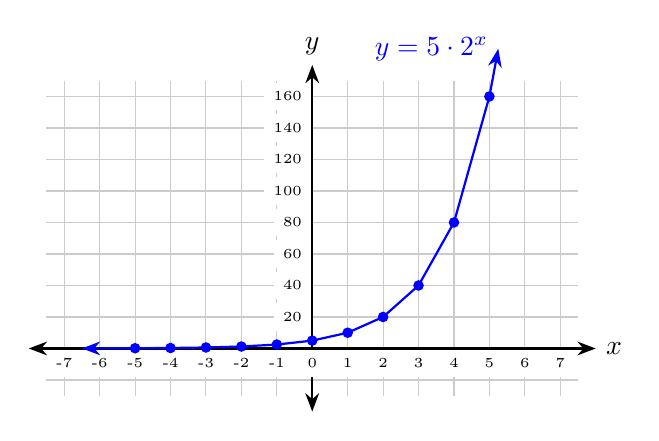
\begin{tikzpicture}
			\begin{scope}[yscale=.02, xscale=.45, >=Stealth, thick]
				\draw[black!20!white, thin, xstep=1, ystep=20] (-7.5, -30) grid (7.5, 170);
				\draw[<->] (0, -40) -- (0,180) node[above] {$y$};
				\draw[<->] (-8, 0) -- (8, 0) node[right] {$x$};
				\foreach \x in {-7,...,7}{
					\node[anchor=north, fill=white, text=black] at (\x, 0) {\tiny\x};
				}
				\foreach \y in {20, 40, 60, 80, 100, 120, 140, 160}{
					\node[anchor=east, fill=white, text=black] at (0, \y) {\tiny\y};
				}
				\pause
				\fill[blue]
					(-5, 0.16125) circle[x radius=.15, y radius=3.375]
					(-4, .3125) circle[x radius=.15, y radius=3.375]
					(-3, .625) circle[x radius=.15, y radius=3.375]
					(-2, 1.25) circle[x radius=.15, y radius=3.375]
					(-1, 2.5) circle[x radius=.15, y radius=3.375]
					(0, 5) circle[x radius=.15, y radius=3.375]
					(1, 10) circle[x radius=.15, y radius=3.375]
					(2, 20) circle[x radius=.15, y radius=3.375]
					(3, 40) circle[x radius=.15, y radius=3.375]
					(4, 80) circle[x radius=.15, y radius=3.375]
					(5, 160) circle[x radius=.15, y radius=3.375];
				\pause
				\draw[blue]
					(-5, 0.16125) --
					(-4, .3125) --
					(-3, .625) --
					(-2, 1.25) --
					(-1, 2.5) --
					(0, 5) --
					(1, 10) --
					(2, 20) --
					(3, 40) --
					(4, 80) --
					(5, 160);
				\pause
				\draw[->, blue] (5, 160) -- (5.25, 190.273) node[left] {$y=5\cdot 2^x$};
				\draw[->, blue] (-5, .16125) -- (-6.5, 0.020617);
			\end{scope}
		\end{tikzpicture}
		\end{center}
		\vfill
	\end{frame}

%	\begin{frame}{Properties}
%		Basic properties:
%		\begin{itemize}
%			\item Domain is $(-\infty, \infty)$; range is $(0,\infty)$ if $C> 0$, and $(-\infty, 0)$ if $C < 0$
%			\pause\vfill
%			\item Increasing or decreasing, one-to-one, continuous
%			\pause\vfill
%			\item No $x$-intercept; $y$-intercept is $C$
%			\pause\vfill
%			\item Horizontal asymptote at $x = \infty$ if $a < 1$ and at $x =-\infty$ if $a > 1$
%		\end{itemize}
%		\pause\vfill
%		Due to our inherited exponent properties, if $f(x) = C\cdot a^x$, and $g(x) = C\cdot \left(\frac{1}{a}\right)^x$, then
%		\pause\vfill
%		\begin{equation*}
%			f(x) = C\cdot a^x = C\cdot\left(\frac{1}{a}\right)^{-x} = g(-x)
%		\end{equation*}
%		\vfill
%		That is, $g$ is the reflection of $f$ over the $y$-axis.
%	\end{frame}

\end{document}